\documentclass[conference]{IEEEtran}
\IEEEoverridecommandlockouts
% The preceding line is only needed to identify funding in the first footnote. If that is unneeded, please comment it out.
%Template version as of 6/27/2024

\usepackage{cite}
\usepackage{amsmath,amssymb,amsfonts}
\usepackage{algorithmic}
\usepackage{graphicx}
\usepackage{textcomp}
\usepackage{xcolor}
\usepackage{hyperref}
\def\BibTeX{{\rm B\kern-.05em{\sc i\kern-.025em b}\kern-.08em
    T\kern-.1667em\lower.7ex\hbox{E}\kern-.125emX}}
\begin{document}

\title{Transformer Decoder Architektur}

\author{\IEEEauthorblockN{1\textsuperscript{st} Stefan Maier}
\IEEEauthorblockA{\textit{Function and Algorithm} \\
\textit{ZF Lifetec}\\
Alfdorf, Deutschland \\
Stefan.Maier1@zf.com}

}

\maketitle
%Literatur aus AMLundXAI.bib einfügen mit 
\bibliographystyle{IEEEtran}



\begin{abstract}
Große Sprache Modelle (engl. Large Language Models) wie Chat GPT basieren auf der Transformer Architektur neuronaler Netze. Die Transformer Architektur besteht dabei aus einem Encoder- sowie Decoder-Element. In der Wissenschaft und Forschung existieren auch Architekturen welche nur einen Teil eines Transformers zur Lösung eines Problems verwenden. In dieser Arbeit wird genauer auf Transformer Architekturen eingegange, welche lediglich aus dem Decoder Element bestehen. Eine weit Verbreitete Decoder Architektur ist die von Chat GPT verwendete GPT (kurz: Generative Pretrained Transformer) Architektur. Es wird auf die Architektur und die weiter Entwicklung der Architektur eingegangen.
\end{abstract}

\begin{IEEEkeywords}
component, formatting, style, styling, insert.
\end{IEEEkeywords}

\section{Einführung}
Die Verarbeitung von natürlicher Sprache (engl. Natural Language Processing. kurz NLP) ist ein wichtiger und großer Bestandteil der künstlichen Intelligenz Forschung. Die Forschungsbereiche decken dabei ein breites Spektrum an Aufgaben ab, wie z.B. Beantwortung von Fragen, Semantische Ähnlichkeit, Text Generierung, Dokumenten Klassifikation o.ä. Die ersten Fortschritte wurde im NLP Bereich bereits durch statistische Hidden Markov Modelle erzielt. Die Leistung solcher statistischen Modelle ist jedoch begrenzt und konnte die Komplexität der natürlichen Sprache nicht geeignet abbilden. Mit den Entwicklungen im Bereich des Deep-Learnings gelangen entscheidende Schritte in der NLP Forschung. Die Transformer Architektur, und das damit verbundene vortrainieren großer Sprachmodelle wie BERT, GPT,T5 oder RoBERTa haben große Fortschritte gebracht, die sich nicht nur auf die NLP Forschung beschränken sondern in der allgemeinen Gesellschaft und Wirtschaft Einzug halten.

\subsection{Ziel der Arbeit}
Das Ziel der Arbeit ist es die Decoder Architektur welche Häufig von generativen Sprachmodellen verwendet wird genauer zu beleuchten. Dabei wird die Decoder-only Architektur anhand des Generative Pretrained Transformers erklärt. Neben dem Generative Pretrained Transformer existieren ebenfalls weitere Modelle die kurz erläutert werden. Weiterhin soll die Arbeit die Anwendungsgebiete sowie Potenziale und Grenzen der Decoder Architektur aufzeigen. Im Ausblick wird auf aktuelle Forschungsfelder im Bereich der Decoder Architekturen eingegangen.
\subsection{Aufbau und Struktur der Arbeit}
Die Arbeit ist wie folgt strukturiert: In Kapitel 2 wird zunächst auf die Grundlagen in Form der Decoder Architektur als Teil der Transformer Architektur eingegangen. Dazu wird die historische Entwicklung, der Aufbau und der Trainingsprozess der Decoder Architektur erläutert und diese vom Encoder Teil der Transformer Architektur abgegrenzt. In Kapitel 3 wird auf unterschiedliche mögliche Anwendungsgebiete aus der Forschung und Entwicklung eingegangen. Aus diesen Erkenntnissen werden in Kapitel 4 die Potenziale und damit einhergehenden Grenzen solcher großen Sprachmodelle eingegangen. Kapitel 5 fasst die Ergebnisse zusammen und gibt einen Ausblick auf die aktuellen Forschungsbereiche.
\section{Decoder Architektur}
Im folgenden Abschnitt wird die Decoder Architektur am Beispiel des Generative Pretrained Transformers (GPT) erläutert. Dabei wird auf die historische Entwicklung, den Aufbau, den Trainingsprozess und die Abgrenzung zur Encoder Architektur eingegangen.
\subsection{Historische Entwicklung der GPT-Decoder Architektur}
Transformer bilden das Grundgerüst moderne großer Sprachmodelle. Diese wurden 2017 in \cite{vaswaniAttentionAllYou2023}  beschrieben. 2018 wurde die erste Version von GPT veröffentlicht, welche auf dem Decoder Part der Transformer Architektur aufbaut. Auf Basis der GPT Modell entstanden weitere Decoder-only Modelle welche die folgende \autoref{fig:Historie} gut veranschaulicht.
\begin{figure}[htbp]
    \centerline{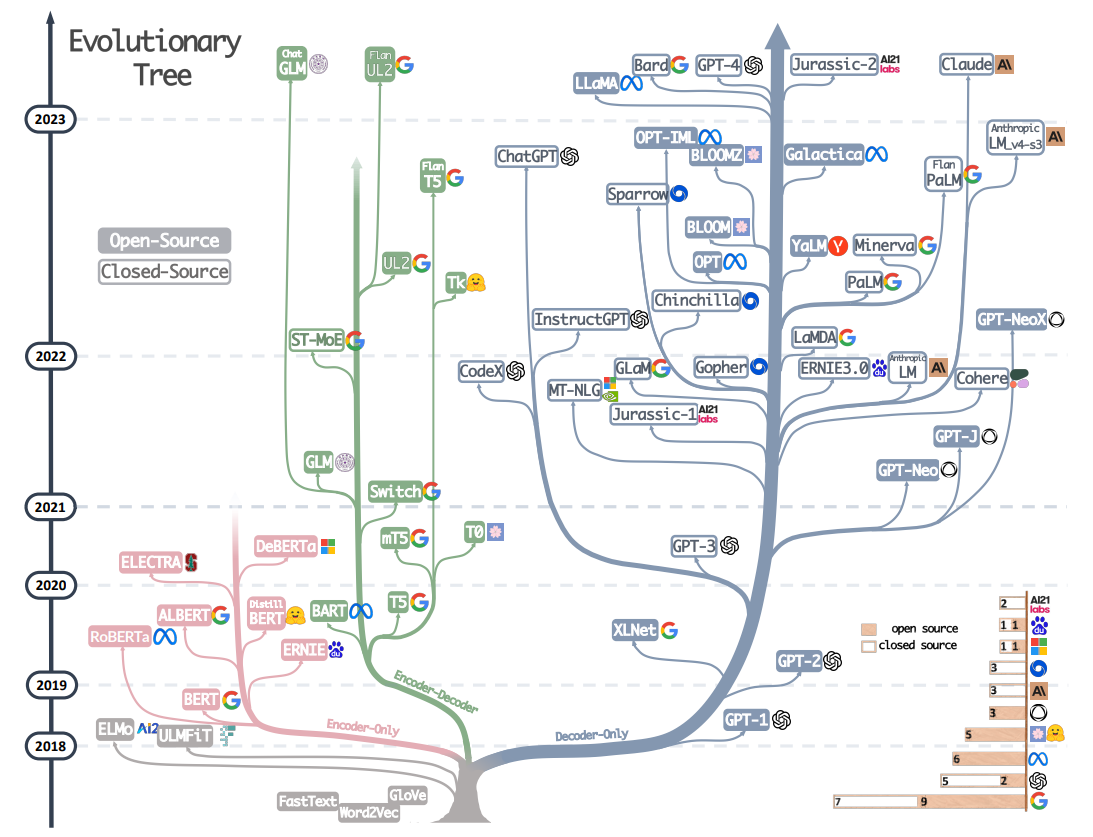
\includegraphics[width=\linewidth]{Bilder/EntwicklungLLM.png}}
    \caption{Historische Entwicklung von Transformer Modellen aus \cite{yangHarnessingPowerLLMs}}
    \label{fig:Historie}
\end{figure}
Die \autoref{fig:Historie} zeigt die Entwicklung unterschiedlicher Transformer Modell bis zum letzten Jahr. Im Rahmen dieser Seminararbeit zeigt Decoder-Only Zweig die Entwicklung von reinen Decoder Architekturen. Damit ist GPT1 eines der ersten Modelle welche auf eine reine Decoder Architekutur setzt. Daraus entsprange viele unterschiedliche Decoder-Only Modelle von Google, Meta oder anderen Forschungseinrichtungen. Die aktuellsten versionen von Llama, GPT-4 oder Bard stellen dabei bis heute die neusten Entwicklungen dar.
\subsection{Aufbau der GPT-Decoder Architektur}
Wie im vorherigen Abschnit beschrieben legt das GPT Modell den Grundstein für die Decoder-only Architektur Entwicklungen. Dies wurde durch das Paper \cite{radfordImprovingLanguageUnderstanding} beschrieben und basiert dabei auf den Grundzügen der Transformer Architekturen welche bereits in Paper \cite{vaswaniAttentionAllYou2023} beschrieben wurden. Die 
folgende Abbildung illustriert dabei den Aufbau einer Decoder Schicht des GPT Modells.
\begin{figure}[htbp]
    \centerline{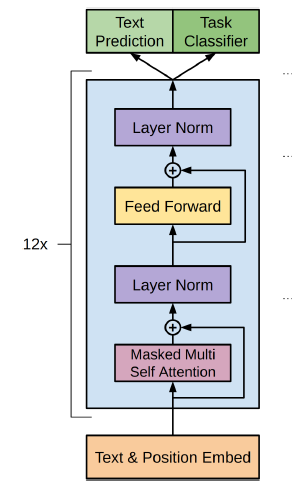
\includegraphics[width=0.4\linewidth]{Bilder/DecoderArchitekturGPT.png}}
    \caption{Decoder Architektur nach \cite{radfordImprovingLanguageUnderstanding}}
    \label{fig:DecoderArchitektur}
\end{figure}
Die \autoref{fig:DecoderArchitektur} zeigt dabei die Architektur Elemente einer Decoder Schicht. Diese Schichten werden in der ersten GPT Architektur 12 mal hintereinander geschaltet. Jedes dieser Decoder Schichten besteht dabei aus einem Masked Multi-Self Attention Layer, Feed Forward Netzwerken, sowie Add und Layer Normalisation Schicht um die Residual Verbindungen der vorherigen Schicht hinzuzufügen. Die Residual Verbindungen sollen vorallem das Problem der verschwindend Gradienten beheben. Der wichtigste Bestandteil der Decoder Schicht ist dabei das Masked Multi-Self Attention Layer. Das Masked Multi-Self Attention Layer ist dabei eine leichte Abwandlung des Mult Self Attention Layers das auch in Encoder Elementen verwendet wird. Nachffolgende Abbildung zeigt den Aufbau eines Multi-Self Attention Layers.
% Neues Bild
\begin{figure}[htbp]
    \centerline{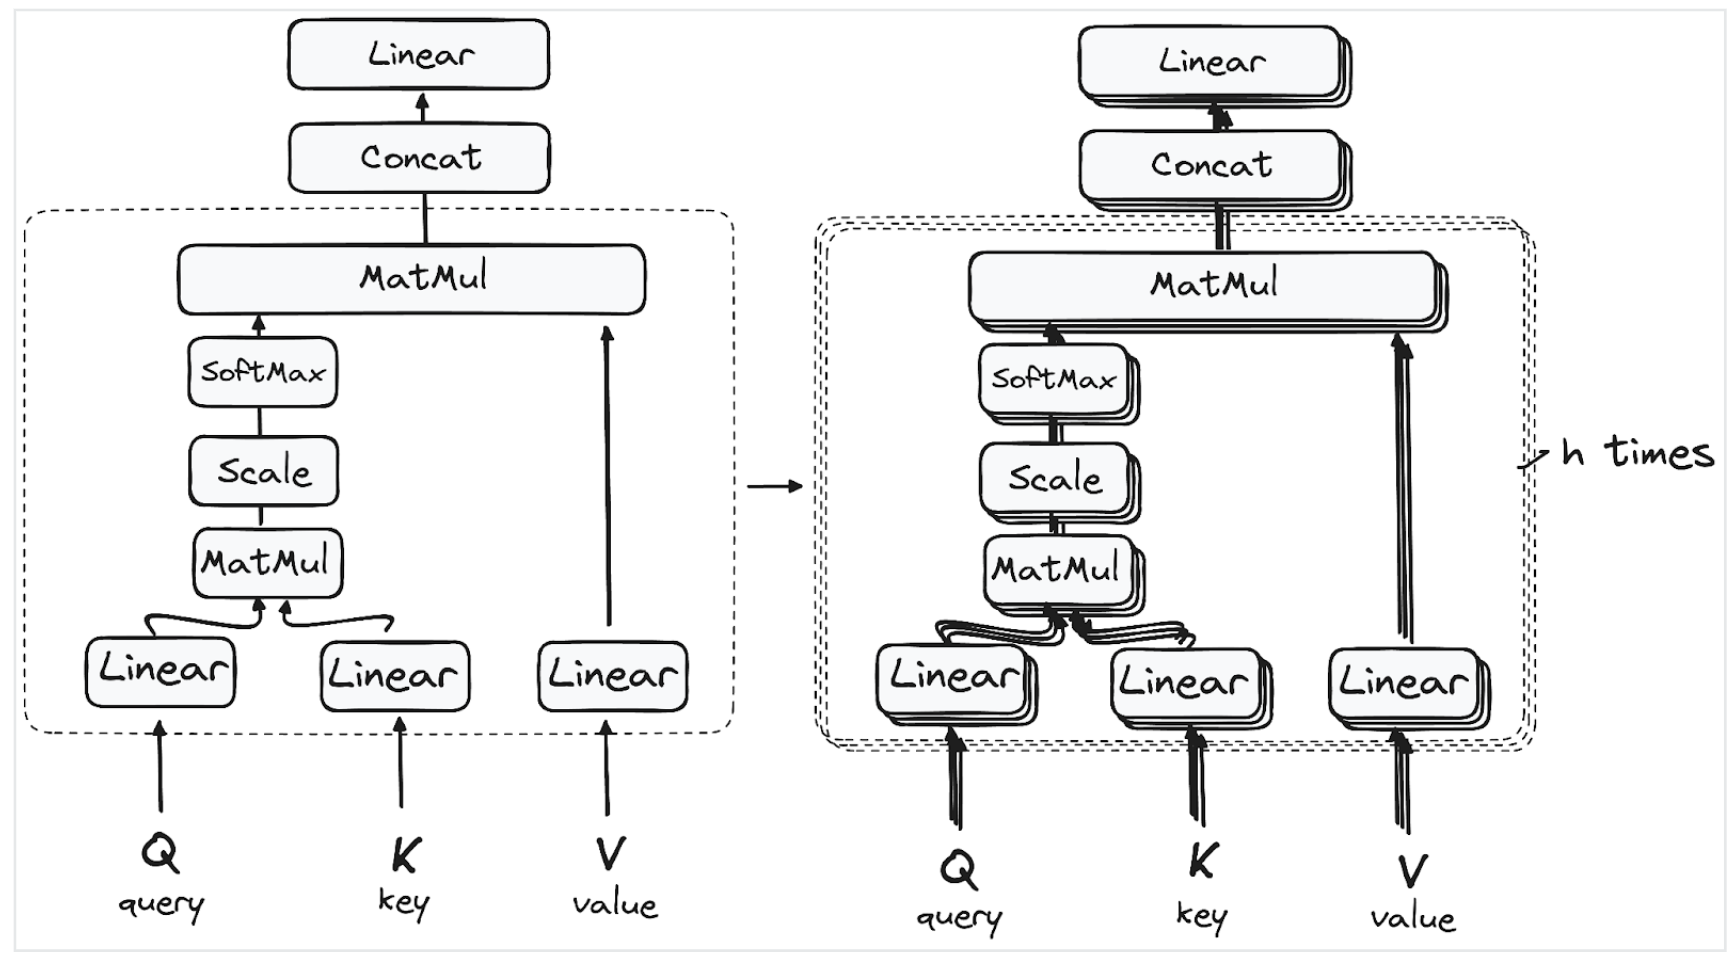
\includegraphics[width=\linewidth]{Bilder/MultiheadSelfAttention.png}}
    \caption{Multi-Self Attention Layer nach \cite{}}
\label{fig:MultiSelfAttention}
\end{figure}
Die Multiplen Heads in der \autoref{fig:MultiSelfAttention} repräsentieren dabei die Anzahl der Köpfe die in der Attention Schicht verwendet werden welche durch die Anzahl an $h$ Köpfe an parallelen Berechnung des Attention Layers bestimmt sind.
zur Berechnung der Ausgabe des Attention Layers werden die Attention Weights berechnet welche bestimen wie wichtig ein Wort für ein anderes Wort ist, was durch nachfolgende Abbildung Visualisiert ist.
% Bild AttentionMechanismus
\begin{figure}[htbp]
    \centerline{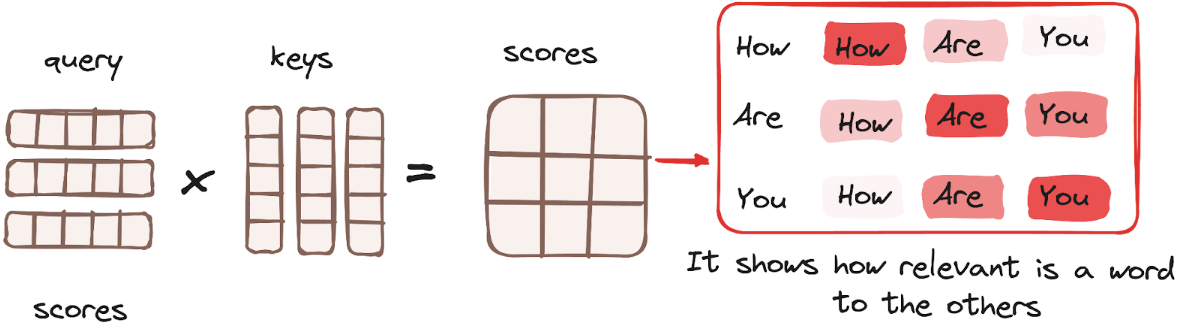
\includegraphics[width=\linewidth]{Bilder/AttentionMechanismus.png}}
    \caption{Attention Mechanismus nach \cite{}}
\label{fig:AttentionMechanismus}
\end{figure}
Die Färbung in der \autoref{fig:AttentionMechanismus} zeigt dabei die Wichtigkeit der Wörter zueinander. Die daraus berechnete Attention Weights werden mit dem Werten der Wörter multipliziert und über ein Lineares Layer verfeinert, dies ergibt die Ausgabe des Attention Layers. Der wesentliche Unterschied zwischen dem Multi-Self Attention Layer und dem Masked Multi-Self Attention Layer ist dabei die Maskierung der Attention Weights. Die Maskierung sorgt dafür, dass ein Wort nur von vorherigen Wörtern abhängt und damit die Attention einbezieht. Die nachfolgende Abbildung zeigt die Maskierung der Attention Weights mithilfe eine Maskierungsmatrix.
% Bild Maskierung

\begin{figure}[htbp]
    \centerline{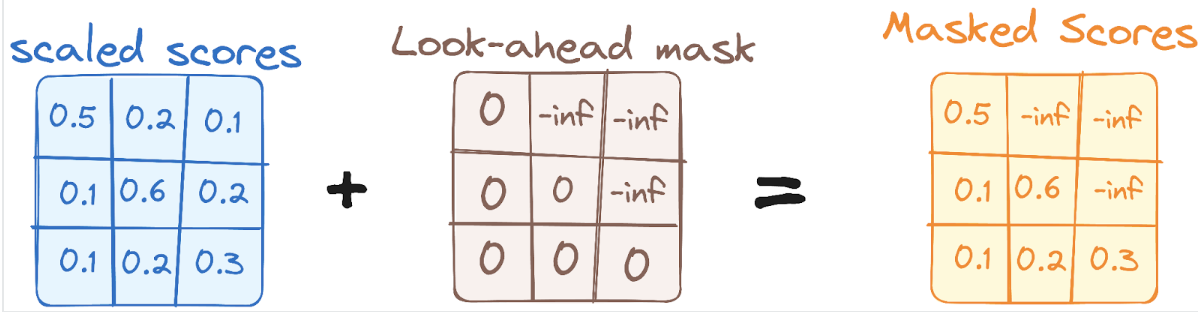
\includegraphics[width=\linewidth]{Bilder/MaskierungAttentionWeights.png}}
    \caption{Maskierung der Attention Weights nach \cite{}}
\label{fig:Maskierung}
\end{figure}
Die genaue Funktionsweise der einzelnen Schichten aus \autoref{fig:DecoderArchitektur}  wird in \cite{vaswaniAttentionAllYou2023} beschrieben. Abschlißend wird in der GPT Architektur ein Layer je nach Aufgabe angehängt, welche in \autoref{fig:DecoderArchitektur} durch Text Vorhersage oder Aufgaben Klassifizierung repräsentiert wird. Dies kann beispielsweise ein Lineares Layer mit Softmax Aktivierungsfunktion sein, welches die Wahrscheinlichkeiten für das nächste Wort aus dem Vokabular berechnet.
\subsection{Abgrenzung der Decoder Architektur zur Encoder Architektur}
Die vorgeschlagende Decoder Architektur durch \cite{radfordImprovingLanguageUnderstanding} unterscheidet sich dabei von der Encoder Architektur durch die Verwendung von Masked Multi-Self Attention Layern. Die Encoder Architektur verwendet hingegen Multi-Self Attention Layer ohne Maskierung. Entscheidend ist ebenfalls das die Architektur aus \cite{radfordImprovingLanguageUnderstanding} keine einzeziehung der Encoder Schicht vorsieht und somit im Vergleich zur Decoder Architektur aus \cite{vaswaniAttentionAllYou2023} keine weitere Multi-Self Attention Layer enthält. Die Decoder Architektur ist dabei auf die Generierung von Text ausgelegt und kann somit als autoregressives Modell betrachtet werden. Die Encoder Architektur hingegen ist auf die Verarbeitung von Texten ausgelegt und kann als diskriminatives Modell betrachtet werden.
\subsection{Trainingsprozess der GPT-Decoder Architektur}
Das entscheidende bei der in \cite{radfordImprovingLanguageUnderstanding} beschrieben Decoder Architektur ist das sogenannte vortrainieren des Modells. Das Vortrainieren des Modells erfolgt dabei auf großen Textkorpora wie Wikipedia, Bücher oder Nachrichten.

\section{Anwendungsbereiche}

\section{Potenzial und Grenzen von Decoder Architekturen}


\section{Fazit}
\subsection{Aktuelle Forschungbereiche}
\subsection{Ausblick}




\bibliography{AMLundXAI}


\end{document}
